\chapter{绘图功能}\label{chap:graphics}
\addtocontents{los}{\protect\addvspace{10pt}}

\begin{intro}
除了排版文字,\LaTeX{} 也支持用代码表示图形。不同的扩展已经极大地丰富了 \LaTeX{} 的图形功能,\hologo{TikZ} 就是其中之一。
本章将带你了解一些基本的绘图功能。

一些特殊的绘图,如交换图、树状图甚至分子式和电路图也能够通过代码绘制,
不过其复杂程度已经超出本手册范围,有兴趣的读者可以查阅一些帮助文档,或者在互联网寻求帮助。
\end{intro}

\section{绘图语言简介}\label{sec:pict-lang}

\LaTeX{} 提供了原始的 \env{picture} 环境,能够绘制一些基本的图形如点、线、矩形、圆、B\'ezier 曲线等等,
不过受制于 \LaTeX{} 本身,它的绘图功能极为有限,效果也不够美观。

当前较为流行的、用于 \LaTeX{} 的绘图宏包 / 程序主要有:
\begin{itemize}
  \item PSTricks \par
  以 PostSciprt 语法为基础的绘图宏包,具有优秀的绘图能力。它对老式的 \texttt{latex + dvips} 编译命令支持最好,
  而现在的几种编译命令下使用起来都不够方便。

  \item \hologo{TikZ} \& \pkg{pgf} \par
  德国的 Till Tantau 教授在开发著名的 \LaTeX{} 幻灯片文档类 \cls{beamer} 时一并开发了绘图宏包 \pkg{pgf},
  目的是令其能够在 \texttt{pdflatex} 或 \texttt{xelatex} 等不同的编译命令下都能使用。
  \hologo{TikZ} 是在 \pkg{pgf} 基础上封装的一个宏包,采用了类似 \hologo{METAPOST} 的语法,提供了方便的绘图命令,绘图能力不输 PSTricks。

  \item \hologo{METAPOST} \& Asymptote \par
  \hologo{METAPOST} 脱胎于高德纳为 \TeX{} 配套开发的字体生成程序 \hologo{METAFONT},
  具有优秀的绘图能力,并能够调用 \TeX{} 引擎向图片中插入文字和公式。
  Asymptote 在 \hologo{METAPOST} 的基础上更进一步,具有一定的类似 C 语言的编程能力,支持三维图形的绘制。\par
  它们作为独立的程序,通常的用法是将代码写在单独的文件里,编译生成图片供 \LaTeX{} 引用,也可以借助特殊的宏包在 \LaTeX{} 代码里直接使用。
\end{itemize}

本手册将介绍 \hologo{TikZ} 绘图宏包里最基本的部分。\hologo{TikZ} 还支持各种自定义的扩展,基于 \hologo{TikZ} 的专门用途的绘图宏包也不胜枚举,
其复杂程度已远远超出入门手册的范围(\hologo{TikZ} 的帮助文档有上千页之厚)。
对此感兴趣的读者需要自行查阅帮助文档,或者到互联网上参考现成的范例。

\section{\hologo{TikZ} 绘图语言}\label{sec:tikz}

\index{TikZ@\protect\hologo{TikZ}}
\pkgindex{tikz}
\envindex[tikz]{tikzpicture}
\cmdindex[tikz]{tikz}
在导言区调用 \pkg{tikz} 宏包,就可以用以下命令和环境使用 \hologo{TikZ} 的绘图功能了%
\footnote{\texttt{latex + dvipdfmx} 编译方式要在 \pkg{tikz} 宏包之前调用 \pkg{graphicx} 宏包并指定 \texttt{dvipdfmx} 选项。}:
\begin{command}
\cmd{tikz}\oarg*{...} \Arg{tikz code}\texttt{;} \\[1ex]
\cmd{tikz}\oarg*{...} \marg*{\Arg{tikz code 1}\texttt{;} \Arg{tikz code 2}\texttt{;} ...} \\[1ex]
\cmd{begin}\marg*{tikzpicture}\oarg*{...} \\
\Arg{tikz code 1}\texttt{;} \\
\Arg{tikz code 2}\texttt{;} \\
... \\
\cmd{end}\marg*{tikzpicture}
\end{command}

前一种用法为 \cmd{tikz} 带单条绘图命令,以分号结束,一般用于在文字之间插入简单的图形;
后两种用法较为常见,使用多条绘图命令,可以在 \env{figure} 等浮动体中使用。

\subsection{\hologo{TikZ} 坐标和路径}\label{subsec:tikz-path}

\hologo{TikZ} 用直角坐标系或者极坐标系描述点的位置。
\begin{itemize}
  \item 直角坐标下,点的位置写作 \texttt{(\Arg{$x$},\Arg{$y$})},坐标 \Arg{$x$} 和 \Arg{$y$} 可以用 \LaTeX{} 支持的任意单位表示,
  缺省为 \texttt{cm};
  \item 极坐标下,点的位置写作 \texttt{(\Arg{$\theta$}:\Arg{r})}。$\theta$ 为极角,单位是度。
\end{itemize}

\cmdindex[tikz]{coordinate}
我们还可以为某个点命名:\cmd{coordinate} \texttt{(A) at (\Arg{coordinate})}
然后就可以使用 \texttt{(A)} 作为点的位置了。

\begin{example}
\begin{tikzpicture}
\draw (0,0) -- (30:1);
\draw (1,0) -- (2,1);
\coordinate (S) at (0,1);
\draw (S) -- (1,1);
\end{tikzpicture}
\end{example}

坐标的表示形式还包括“垂足”形式:
\begin{example}
\begin{tikzpicture}
\coordinate (S) at (2,2);
\draw[gray] (-1,2) -- (S);
\draw[gray] (2,-1) -- (S);
\draw[red] (0,0) -- (0,0 -| S);
\draw[blue] (0,0) -- (0,0 |- S);
\end{tikzpicture}
\end{example}


\hologo{TikZ} 最基本的路径为两点之间连线,如 \texttt{(\Arg{$x_1$},\Arg{$y_1$}) -{}- (\Arg{$x_2$},\Arg{$y_2$})},可以连用表示多个连线(折线)。
连续使用连线时,可以使用 \texttt{cycle} 令路径回到起点,生成闭合的路径。
\begin{example}
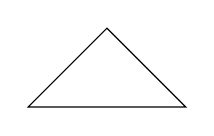
\begin{tikzpicture}
\draw (0,0) -- (1,1) -- (2,0) -- cycle;
\end{tikzpicture}
\end{example}

多条路径可用于同一条画图命令中,以空格分隔:
\begin{example}
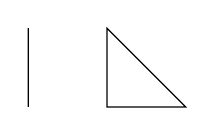
\begin{tikzpicture}
\draw (0,0) -- (0,1)
      (1,0) -- (1,1) -- (2,0) -- cycle;
\end{tikzpicture}
\end{example}

其它常用的路径还包括:
\begin{itemize}
  \item 矩形、圆和椭圆:
\end{itemize}
\begin{example}
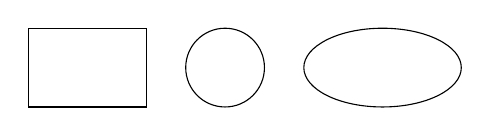
\begin{tikzpicture}
\draw (0,0) rectangle (1.5,1);
\draw (2.5,0.5) circle [radius=0.5];
\draw (4.5,0.5) ellipse
    [x radius=1,y radius=0.5];
\end{tikzpicture}
\end{example}

\begin{itemize}
  \item 直角、圆弧、椭圆弧:
\end{itemize}
\begin{example}
\begin{tikzpicture}
\draw (0,0) |- (1,1);
\draw (1,0) -| (2,1);
\draw (4,0) arc (0:135:1);
\draw (6,0) arc (0:135:1 and 0.5);
\end{tikzpicture}
\end{example}

\begin{itemize}
  \item 正弦、余弦曲线(1/4 周期):
\end{itemize}
\begin{example}
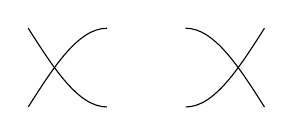
\begin{tikzpicture}
\draw (0,0) sin (1,1);
\draw (0,1) sin (1,0);
\draw (2,1) cos (3,0);
\draw (2,0) cos (3,1);
\end{tikzpicture}
\end{example}

\begin{itemize}
  \item 抛物线,用 \texttt{bend} 控制顶点:
\end{itemize}
\begin{example}
\begin{tikzpicture}
\draw (0,0) parabola (1,2);
\draw (2,0) parabola
      bend (2.25,-0.25) (3,2);
\draw (4,0) parabola
      bend (4.75,2.25) (5,2);
\end{tikzpicture}
\end{example}

\begin{itemize}
  \item 二次和三次 B\'ezier 曲线,分别使用一个和两个控制点:
\end{itemize}
\begin{example}
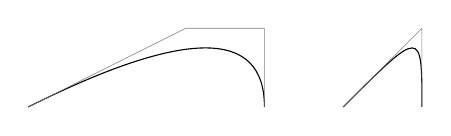
\begin{tikzpicture}
\draw (0,0) .. controls
  (2,1) and (3,1) .. (3,0);
\draw (4,0) .. controls
  (5,1) .. (5,0);
\draw[help lines] (0,0)
  -- (2,1) -- (3,1) -- (3,0)
  (4,0) -- (5,1) -- (5,0);
\end{tikzpicture}
\end{example}

\begin{itemize}
  \item 网格、函数图像,网格可用 \texttt{step} 参数控制网格大小,函数图像用 \texttt{domain} 参数控制定义域:
\end{itemize}
\begin{example}
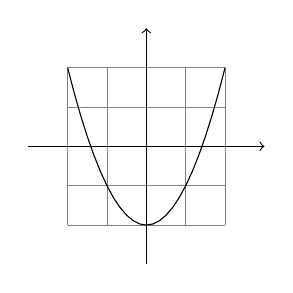
\begin{tikzpicture}
\draw[help lines,step=0.5]
     (-1,-1) grid (1,1);
\draw[->] (-1.5,0) -- (1.5,0);
\draw[->] (0,-1.5) -- (0,1.5);
\draw[domain=-1:1]
     plot(\x,{\x*\x*2 -1});
\end{tikzpicture}
\end{example}

\subsection{\hologo{TikZ} 绘图命令和参数}\label{subsec:tikz-draw}

\cmdindex[tikz]{draw,fill,filldraw}
除了 \cmd{draw} 命令之外,\hologo{TikZ} 还提供了 \cmd{fill} 命令用来填充图形,\cmd{filldraw} 命令则同时填充和描边。
除了矩形、圆等现成的闭合图形外,\cmd{fill} 和 \cmd{filldraw} 命令也能够填充人为构造的闭合路径。
\begin{command}
\cmd{draw}\oarg*{...} \Arg{path}; \\
\cmd{fill}\oarg*{...} \Arg{path}; \\
\cmd{filldraw}\oarg*{...} \Arg{path};
\end{command}

绘图参数可作为可选参数用在 \env{tikzpiture} 环境或 \cmd{tikz} 命令时,参数会影响到所有具体的绘图命令;
用在单个绘图命令 \cmd{draw}、\cmd{filldraw} 等时,只对这个命令起效。

\hologo{TikZ} 有数不清的绘图参数,这些参数令 \hologo{TikZ} 能够绘制丰富多彩的图像,同时也令 \hologo{TikZ} 难以精通。
以下示例常用的一些绘图参数。

\begin{itemize}
  \item \texttt{color/draw/fill=\Arg{color}} 为 \cmd{draw} 或 \cmd{fill} 等命令指定颜色。
  \texttt{draw} 和 \texttt{fill} 分别指定填充和描边的颜色,而 \texttt{color} 同时指定,
  可以省略 \texttt{color=} 直接写颜色名称。
\end{itemize}
\begin{example}

\begin{tikzpicture}[thick]
\draw[blue] (0,0) rectangle (1,1);
\filldraw[fill=yellow,draw=red]
  (2,0.5) circle [radius=0.5];
\end{tikzpicture}
\end{example}

\begin{itemize}
  \item \texttt{thick=\Arg{length}/thin/semithick/...} 指定线条的粗细。
\end{itemize}
\begin{example}

\begin{tikzpicture}
\draw[ultra thin] (0,0)--(0,2);
\draw[very thin] (0.5,0)--(0.5,2);
\draw[thin] (1,0)--(1,2);
\draw[semithick] (1.5,0)--(1.5,2);
\draw[thick] (2,0)--(2,2);
\draw[very thick] (2.5,0)--(2.5,2);
\draw[ultra thick] (3,0)--(3,2);
\end{tikzpicture}
\end{example}

\begin{itemize}
  \item \texttt{solid/dashed/dotted/dash dot/dash dot dot} 指定线条类型(实线、虚线、点划线等)。
  与 \texttt{dashed} 对应地有 \texttt{densely dashed} 和 \texttt{loosely dashed},后三种类型同理。
\end{itemize}
\begin{example}
\begin{tikzpicture}
\draw[dashed] (0,0) -- (0,2);
\draw[dotted] (0.5,0) -- (0.5,2);
\draw[dash dot] (1,0) -- (1,2);
\draw[dash dot dot] (1.5,0) -- (1.5,2);
\draw[densely dotted]
   (2,0) -- (3,2) -- (4,0) -- cycle;
\end{tikzpicture}
\end{example}

\begin{itemize}
  \item \texttt{\Arg{arrow}-\Arg{arrow}} 指定线条首尾的箭头形式。
  复杂的箭头形式需要在导言区使用 \cmd{use\-tikz\-library} \marg*{arrows.meta}。
\end{itemize}
\begin{example}
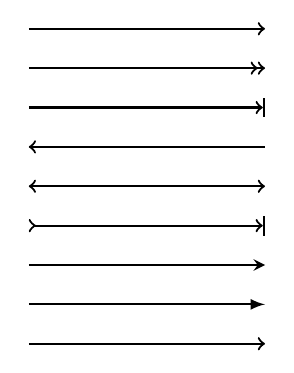
\begin{tikzpicture}[thick]
\draw[->] (0,4) -- (3,4);
\draw[->>] (0,3.5) -- (3,3.5);
\draw[->|] (0,3) -- (3,3);
\draw[<-] (0,2.5) -- (3,2.5);
\draw[<->] (0,2) -- (3,2);
\draw[>->|] (0,1.5) -- (3,1.5);
\draw[-stealth] (0,1) -- (3,1);
\draw[-latex] (0,0.5) -- (3,0.5);
\draw[-to] (0,0) -- (3,0);
\end{tikzpicture}
\end{example}

\begin{itemize}
  \item \texttt{rounded corners\oarg*{=\Arg{radius}}/sharp corners} 将路径转向处绘制成圆角/直角。可选参数 \Arg{radius} 控制圆角的半径。
  可以对某一段路径直接使用。
\end{itemize}
\begin{example}
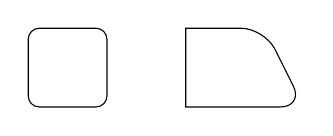
\begin{tikzpicture}
\draw[rounded corners]
  (0,0) rectangle (1,1);
\draw (2,0) -- (2,1)
  [rounded corners=.3cm]
  -- (3,1) -- (3.5,0)
  [sharp corners] -- cycle;
\end{tikzpicture}
\end{example}

\begin{itemize}
  \item \texttt{scale/xshift/yshift/xslant/yslant/rotate} 设定图形的缩放、位移和旋转。
\end{itemize}
\begin{example}
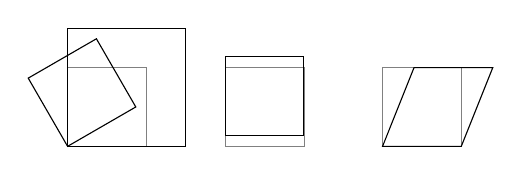
\begin{tikzpicture}
\draw[help lines](0,0) rectangle (1,1);
\draw[scale=1.5] (0,0) rectangle (1,1);
\draw[rotate=30] (0,0) rectangle (1,1);
\draw[help lines](2,0) rectangle (3,1);
\draw[yshift=4pt](2,0) rectangle (3,1);
\draw[help lines](4,0) rectangle (5,1);
\draw[xslant=0.4](4,0) rectangle (5,1);
\end{tikzpicture}
\end{example}

为了重复利用绘图参数,减少代码冗余,\hologo{TikZ} 引入了“样式”的概念,可以定义一个样式包含绘图参数,
然后将样式作为一个参数用于绘图:
\begin{example}
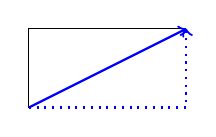
\begin{tikzpicture}
  [myarrow/.style={blue,thick,->}]
\draw (0,0)--(0,1)--(2,1);
\draw[myarrow] (0,0)--(2,1);
\draw[myarrow,dotted]
  (0,0)--(2,0)--(2,1);
\end{tikzpicture}
\end{example}

\envindex[tikz]{scope}
\hologo{TikZ} 还提供了 \env{scope} 环境,令绘图参数或样式在局部生效:
\begin{example}
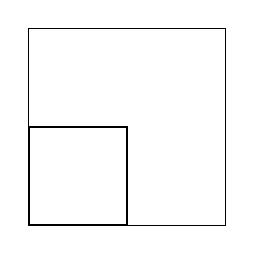
\begin{tikzpicture}
\draw (0,0) rectangle (2.5, 2.5);
\begin{scope}[thick,scale=0.5]
\draw (0,0) rectangle (2.5, 2.5);
\end{scope}
\end{tikzpicture}
\end{example}

\subsection{\hologo{TikZ} 文字结点}\label{subsec:tikz-node}

\cmdindex[tikz]{node}
\hologo{TikZ} 用 \cmd{node} 命令绘制文字结点:
\begin{command}
\cmd{node}\oarg{options} \texttt{(\Arg{name})} \texttt{at (\Arg{coordinate})} \marg{text}\texttt{;}
\end{command}
\texttt{(\Arg{name})} 为结点命名,类似 \cmd{coordinate};\texttt{at (\Arg{coordinate})} 指定结点的位置。
这两者和前面的 \Arg{options} 都可以省略,只有 \Arg{text} 是必填的。
\begin{example}
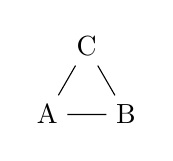
\begin{tikzpicture}
\node (A) at (0,0) {A};
\node (B) at (1,0) {B};
\node (C) at (60:1) {C};
\draw (A) -- (B) -- (C) -- (A);
\end{tikzpicture}
\end{example}

\ref{subsec:tikz-draw} 小节中的参数可用于 \cmd{node} 命令的配置。除此之外,\cmd{node} 还有一些特定的参数:
\begin{itemize}
  \item \texttt{anchor=\Arg{position}} 令结点的某个角落 \Arg{position} 与 \Arg{coordinate} 对应。
  \item \texttt{centered / above / below / left / right / above left / ... \oarg*{=\Arg{length}}} \\
  与 \texttt{anchor} 等效的选项。可选的 \Arg{length} 为节点相对于 \Arg{coordinate} 的距离。
\end{itemize}
\begin{example}
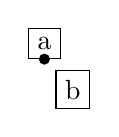
\begin{tikzpicture}
\coordinate (A) at (1,1);
\fill (A) circle[radius=2pt];
\node[draw,anchor=south] at (A) {a};
\node[draw,below right=4pt] at (A) {b};
\end{tikzpicture}
\end{example}

\begin{itemize}
  \item \texttt{shape=\Arg{shape}}
  结点的形状,默认可用 \texttt{rectangle} 和 \texttt{circle},可省略 \texttt{shape=} 直接写。在导言区使用命令
  \cmd{use\-tikz\-library}\marg*{shapes.geometric} 可用更多的形状。
  \item \texttt{text=\Arg{color}}
  结点文字的颜色。
  \item \texttt{node font=\Arg{font command}}
  结点文字的字体,形如 \cmd{bfseries} 或 \cmd{itshape} 等。
\end{itemize}
\begin{example}
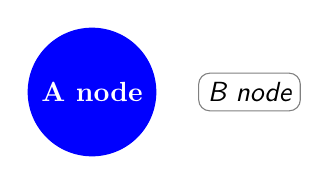
\begin{tikzpicture}
\node[circle,fill=blue,text=white,
  node font={\bfseries}]
  (A) at (0,0) {A node};
\node[rectangle,rounded corners,
  draw=gray,
  node font={\sffamily\slshape}]
  (B) at (2,0) {B node};
\end{tikzpicture}
\end{example}

\begin{itemize}
  \item \texttt{inner sep=\Arg{length} / outer sep=\Arg{length}}
  结点边界向外和向内的额外距离。
  \item \texttt{minimum size=\Arg{length} / minimum height=\Arg{length} / minimum width=\Arg{length}} \\
  结点的最小大小或最小高度/宽度。
\end{itemize}

\cmd{node} 命令不仅为文字结点的位置命名,在 \cmd{draw} 等命令中还可以使用某个结点的相对位置,
以“东南西北”的方式命名:
\begin{example}
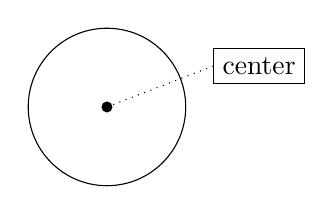
\begin{tikzpicture}
\draw (0,0) circle[radius=1];
\fill (0,0) circle[radius=2pt];
\node[draw] (P) at (15:2) {center};
\draw[dotted] (0,0) -- (P.west);
\end{tikzpicture}
\end{example}

\cmd{node} 命令的一种等效用法是在 \cmd{draw} 等命令的路径中使用 \texttt{node},不仅可以对某个位置标记节点,还能够对线标记:
\begin{example}
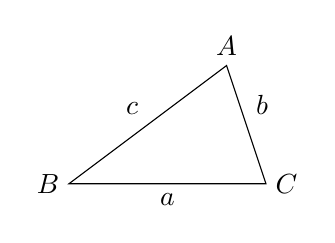
\begin{tikzpicture}
\draw (2,1.5) node[above] {$A$}
       -- node[above left]  {$c$}
    (0,0) node[left]  {$B$}
       -- node[below]       {$a$}
  (2.5,0) node[right] {$C$}
       -- node[above right] {$b$}
       cycle;
\end{tikzpicture}
\end{example}

在此举一个较为复杂的例子,综合前面介绍过的各种路径、形状、文字结点和参数设置,见源代码 \ref{code:tikz-example}。

\begin{sourcecode}[htp]
\begin{Verbatim}
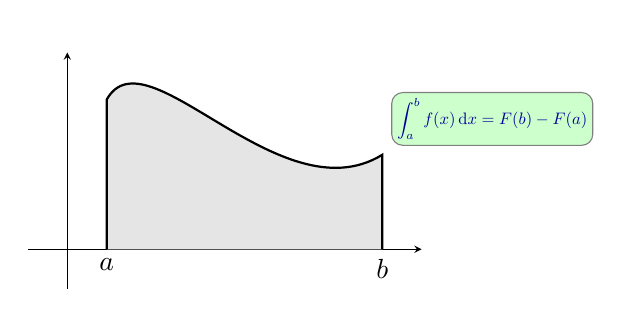
\begin{tikzpicture}
\draw[-stealth,line width=0.2pt] (-0.5,0) -- (4.5,0);
\draw[-stealth,line width=0.2pt] (0,-0.5) -- (0,2.5);
\coordinate (a)  at (0.5,1.9);
\coordinate (b)  at (4,1.2);
\node[below] (a0) at (a |- 0,0) {$a$};
\node[below] (b0) at (b |- 0,0) {$b$};
\filldraw[fill=gray!20,draw,thick]
  (a0) -- (a) .. controls (1,2.8) and (2.7,0.4) .. (b) -- (b0) -- cycle;
\node[above right,outer sep=0.2cm, rounded corners,
  fill=green!20,draw=gray,text=blue!60!black,scale=0.6]
  at (b) {$\displaystyle \int_a^b {f(x)\,\mathrm{d}x} = F(b) - F(a)$};
\end{tikzpicture}
\end{Verbatim}
\begin{center}
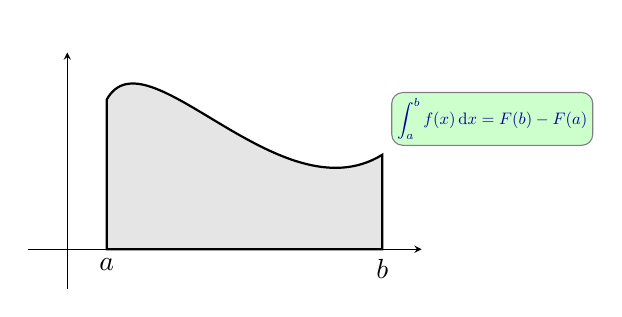
\begin{tikzpicture}
\draw[-stealth,line width=0.2pt] (-0.5,0) -- (4.5,0);
\draw[-stealth,line width=0.2pt] (0,-0.5) -- (0,2.5);
\coordinate (a)  at (0.5,1.9);
\coordinate (b)  at (4,1.2);
\coordinate[label=below:$a$] (a0) at (a |- 0,0);
\coordinate[label=below:$b$] (b0) at (b |- 0,0);
\filldraw[fill=gray!20,draw,thick]
  (a0) -- (a) .. controls (1,2.8) and (2.7,0.4) .. (b) -- (b0) -- cycle;
\node[above right,outer sep=0.2cm, rounded corners,
  fill=green!20,draw=gray,text=blue!60!black,scale=0.6]
  at (b) {$\displaystyle \int_a^b {f(x)\,\mathrm{d}x} = F(b) - F(a)$};
\end{tikzpicture}
\end{center}
\caption{\hologo{TikZ} 绘图示例源代码和效果。}\label{code:tikz-example}
\end{sourcecode}

\subsection{在 \hologo{TikZ} 中使用循环}

\cmdindex[tikz]{foreach}
\hologo{TikZ} 通过 \pkg{pgffor} 功能宏包实现了简单的循环功能,语法为:
\begin{command}
\cmd{foreach} \cmd{a} \texttt{in} \marg{list} \marg{commands}
\end{command}
上述语法定义了 \cmd{a} 为变量,在 \marg{commands} 中使用 \cmd{a} 完成循环。

\Arg{list} 可以直接将所有值写出来,如 1,2,3,4;也可以写成省略形式,如 1,2,\ldots,10。
\begin{example}
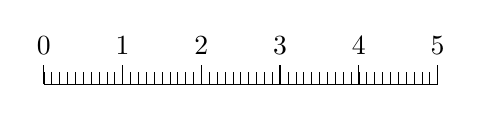
\begin{tikzpicture}
\draw (0,0)--(5,0);
\foreach \i in {0.0,0.1,...,5.0}
  {\draw[very thin]
     (\i,0)--(\i,0.15);}
\foreach \I in {0,1,2,3,4,5}
  {\draw (\I,0)--(\I,0.25)
     node[above] {\I};}
\end{tikzpicture}
\end{example}

\cmd{foreach} 还可使用变量对参与循环:
\begin{example}
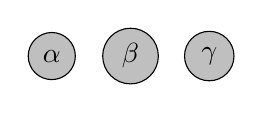
\begin{tikzpicture}
\foreach \n/\t in
  {0/\alpha,1/\beta,2/\gamma}
  {\node[circle,fill=lightgray,draw]
    at (\n,0) {$\t$};}
\end{tikzpicture}
\end{example}

\endinput
